% !TeX spellcheck = en_US
\documentclass[letterpaper,12pt,twoside]{report}
\usepackage{fancyhdr}
\usepackage{fullpage}
\usepackage{tikz}
\usepackage{amsmath}

\begin{document}
	\pagestyle{fancy}
	\fancyhf{}
	\fancyhead[L]{Day 2}
	\fancyhead[R]{\textit{The Calendar Project}}
	\fancyfoot[L]{Citations Involved: none}
	
	% Problem
	\paragraph{Problem}
	\begin{quote}
	\textsf{An \textit{equable} shape is one whose area and perimeter are numerically equal. What are the lengths of the legs of an equable isosceles right triangle?}
	\end{quote}
	
	% Graphics
	\begin{center}
		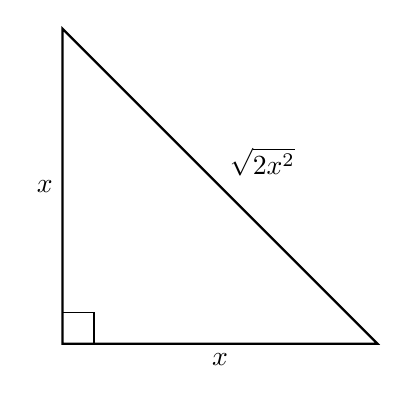
\begin{tikzpicture}
		\draw[thick] (0,4) -- (0,0) -- (4,0) -- cycle;
		\draw (0,0.4) -- (0.4,0.4) -- (0.4,0);
		\node[left] at (0,2) {$x$};
		\node[below] at (2,0) {$x$};
		\node[above right] at (2,2) {$\sqrt{2x^2}$};
		\end{tikzpicture}
	\end{center}
	
	% Reasoning
	\paragraph{Reasoning}
	\begin{quotation}
	
	The triangle area formula is $\frac{1}{2}bh$ (2). For isosceles right triangles, $b=h$ and the formula is specialized to $\frac{1}{2}x^2$ where $x$ is the leg length. Using the Pythagorean Theorem ($a^2+b^2=c^2$) (1), the hypotenuse of the triangle illustrated above can be represented using $\sqrt{x^2+x^2}$. This is simplified to $\sqrt{2x^2}$ and produces the final perimeter formula for this triangle, $2x+\sqrt{2x^2}$. For an equable right isosceles triangle (whose area and perimeter are numerically equal), $\frac{1}{2}x^2 = 2x+\sqrt{2x^2}$ by definition. The following steps solve this equation for $x$.
	
	\begin{center}
		\begin{tabular}{l | l}
			$\frac{1}{2}x^2 = 2x+x\sqrt{2}$ & Split the square root \\
			$\frac{1}{2}x = 2+\sqrt{2}$ & Divide both sides by $x$ \\
			$x = 4+2\sqrt{2}$ & Multiply both sides by 2
		\end{tabular}
	\end{center}

	The final solution is therefore $\boxed{4+2\sqrt{2} \approx 6.83}$.
	
	\end{quotation}
	
	\paragraph{External References}
	
	\begin{enumerate}
		\item Textbook Ch. 9, Pg. 587: Pythagorean Theorem (Theorem 1-6-1)
		\item Textbook Ch. 9, Pg. 590: Area of Triangles and Trapezoids
	\end{enumerate}

\end{document}